\subsection{Muon spectrometer}

Muon spectrometer~\cite{CERN-LHCC-97-022} is the outermost part of the ATLAS detector with an extremely large tracking system.
It measures a large range of muon momentum, and the accuracy is about 3\% at 100 GeV and 10\% at 1 TeV.
The muon spectrometer comprises three main parts: a magnetic field produced by three toroidal magnets;
a set of chambers measuring the tracks of muons with high spatial precision; and triggering chambers with accurate time-resolution. 
Figure~\ref{fig:muon_dec} shows the schematic of ATLAS muon spectrometer that consists of four types of muon chambers 
(\textit{MDT, CSC, RPC, TGC}) as well as the magnet systems (barrel and end-cap toroid).
\begin{figure}[!htb]
  \centering
  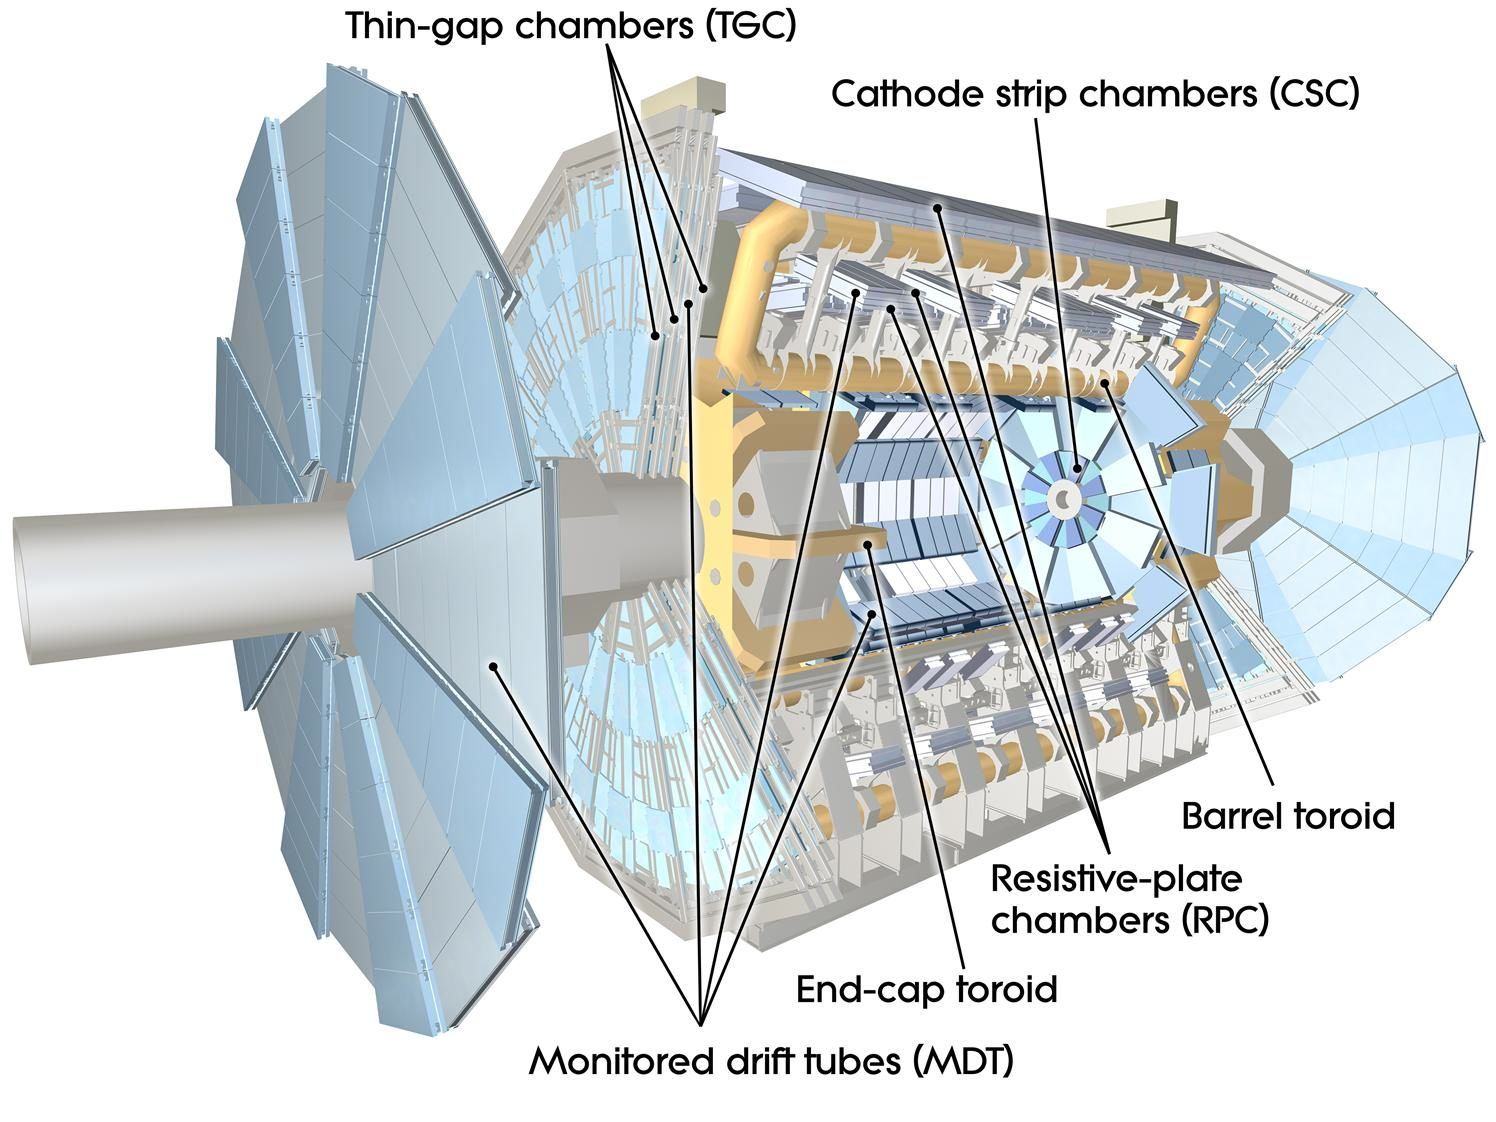
\includegraphics[width=0.8\textwidth]{figures/Detector/muon_all.png}
  \caption{Cut-away view of the ATLAS muon spectrometer\cite{Sliwa:2013oua}.}
  \label{fig:muon_dec}
\end{figure}

More details of four chambers are given as below:
\begin{itemize}
	\item \textbf{Monitored Drift Tubes (MDT)}. MDTs provide the precise momentum measurement with the $|\eta|$ range up to 2.7, except in the innermost end-cap layer where the coverage is limited to $|\eta| < 2.0$. The chambers comprises three or four layers of drift tubes, with a diameter of 29.970 mm, operated with Ar/CO2 gas (93/7) at 3 bar. The average resolution can reach 80 $\mu$m per tube and 30 $\mu$m per chamber.
	\item \textbf{Cathode strip chambers (CSC)}. CSCs are used in the forward region of $2 < |\eta| < 2.7$ in the innermost tracking layers, due to their good time resolution and high rate capability. The CSCs are multi-wire proportional chambers (MWPC) with the cathode planes segmented into strips in orthogonal directions, which allows both coordinates to be measured from the induced-charge distribution. The resolution of a chamber is about 40 $\mu$m for bending plane and 5 mm for the transverse plane.
	\item \textbf{Resistive plate chambers (RPC)}. The RPCs serves as fast triggers in the barrel region of $|\eta| < 1.05$ due to the high rate capability and good spatial and time resolution. It is a gaseous parallel electrode-plate detector without any wires. There are three concentric cylindrical layers around the beam axis, as three trigger stations. Each stations consists of two independent layers to measure the transverse coordinates of $\eta$ and $\phi$.
	\item \textbf{Thin gap chambers (TGC)}. TGCs are used as trigger system for the end-cap region of $1.5 < |\eta| < 2.4$, and works based on the same principle as multi-wire proportional chambers. In addition, they can also provide the second azimuthal coordinate to complement the measurement of MDT in bending direction.
\end{itemize}
